\section*{Задание 1. Измерение периода колебаний, логарифмического декремента
и параметров контура}

Измерим амплитуды колебаний, отстоящих друг от друга на $n = 5,\ldots,15$
и вычислим логарифмический декремент по формуле (\ref{7a}).

По формулам $\delta = \frac\lambda t$, $Q = \frac\pi\lambda$ и $\tau=\frac1\lambda$
рассчитаем коэффициент затухания, добротность и время релаксации.

$С$ находится из модифицированной формулы (\ref{5}):
\begin{equation}
	\label{C}
	C = \frac{
		4LT^2
	}{
		16\pi^2L^2+R^2T^2
	}
\end{equation}

Повторим измерения для других значений внешнего сопротивления $R_m$ в 
интервале от 1 до 10 Ом.

Построим график зависимости $\lambda(R_m)$. Эту зависимость можно 
аппроксимировать линейной функцией $y = A + Bx$. Проведя прямую (построенную
с помощью метода наименьших квадратов) до 
пересечения с $\lambda = 0$, найдём эквивалентное сопротивление 
контура $R_k = 22,16$.

\begin{center}
	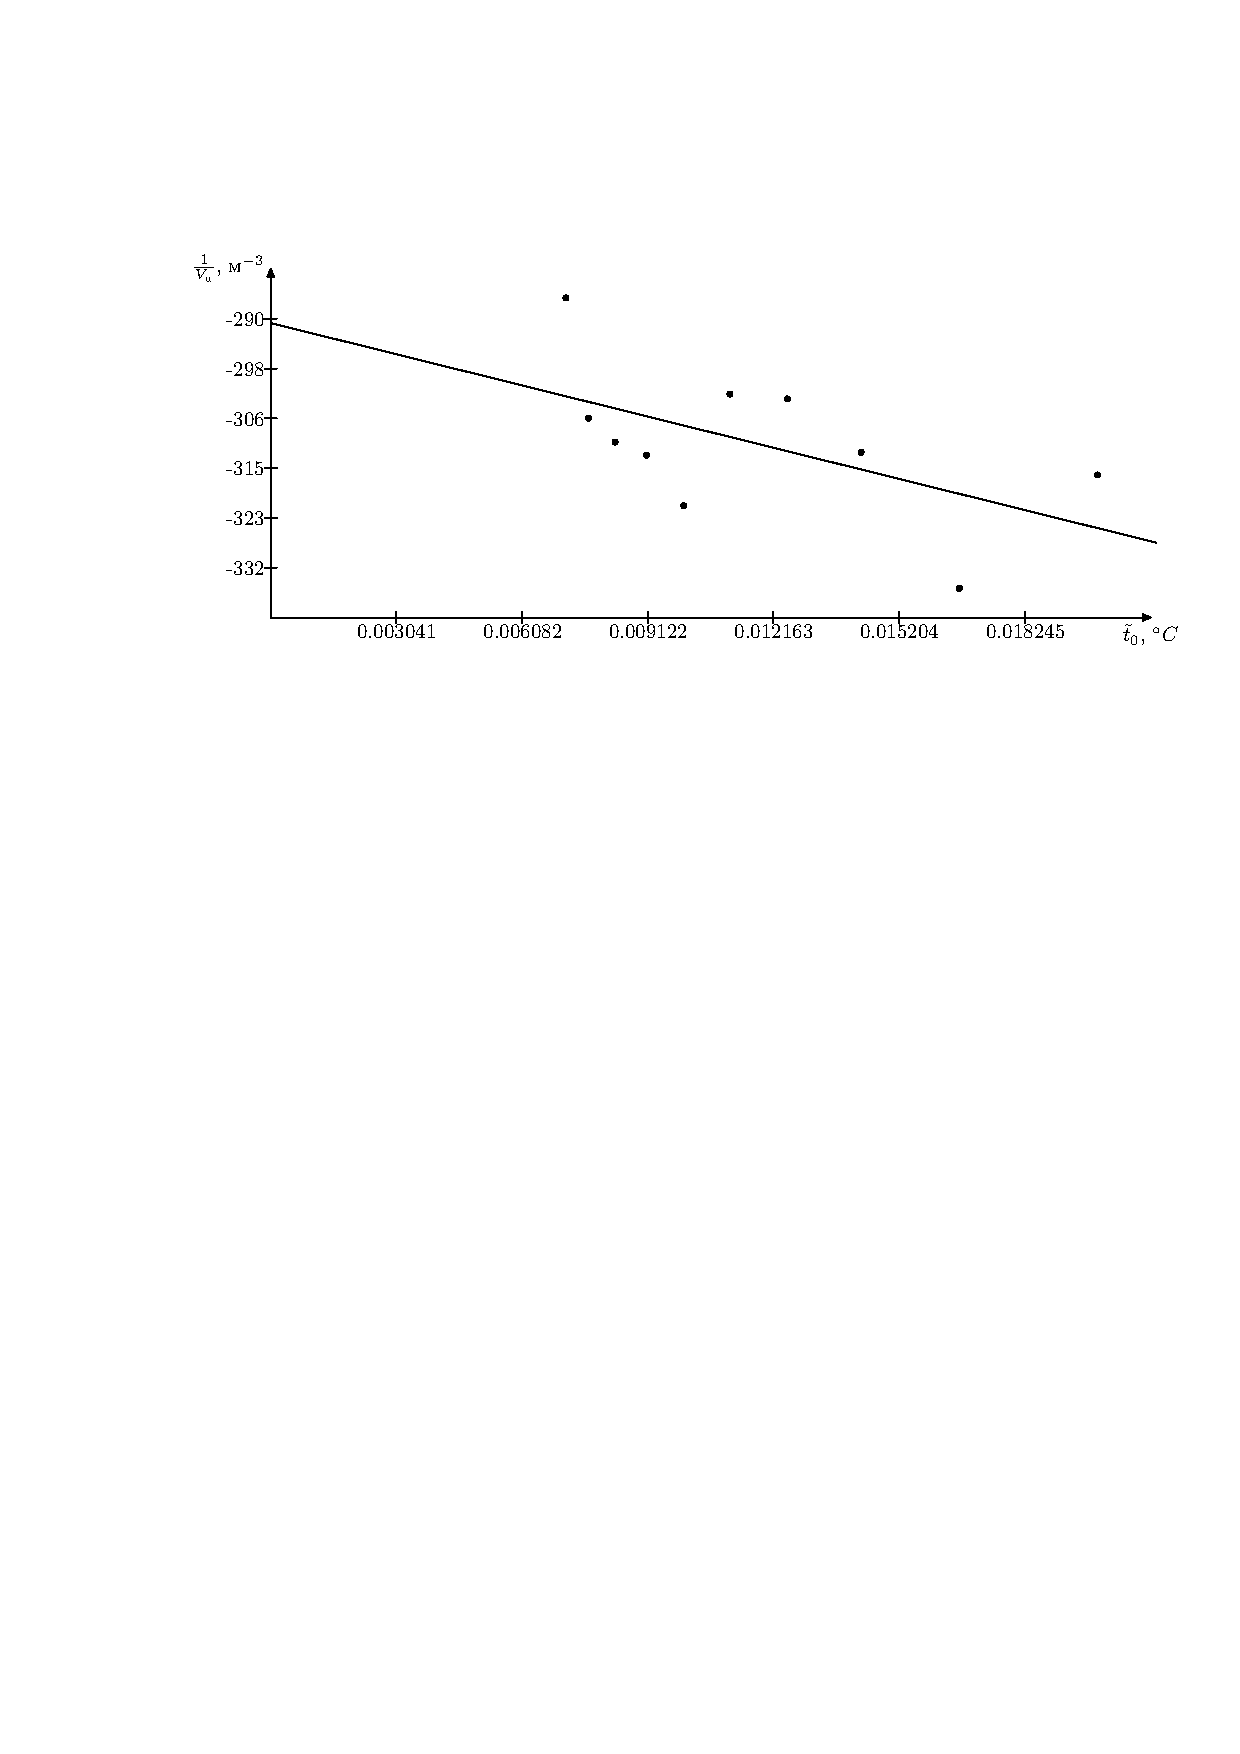
\includegraphics[scale=0.13]{pics/png/points4.png}
\end{center}

\begin{tabular}{|c|c|c|c|c|c|c|c|c|}
\hline
$\No$ & 1 & 2 & 3 & 4 & 5 & 6 & 7 & 8\\
\hline
$X$ & 2 & 4 & 6 & 8 & 10 & 12 & 14 & 16\\
\hline
$\phi$ & 8,75 & 7,5 & 6,35 & 5,2 & 4,1 & 3,05 & 2,01 & 1\\
\hline
\\
\hline
\end{tabular}
\par

